\documentclass[twoside]{book}

% Packages required by doxygen
\usepackage{calc}
\usepackage{doxygen}
\usepackage{graphicx}
\usepackage[utf8]{inputenc}
\usepackage{makeidx}
\usepackage{multicol}
\usepackage{multirow}
\usepackage{fixltx2e}
\PassOptionsToPackage{warn}{textcomp}
\usepackage{textcomp}
\usepackage[nointegrals]{wasysym}
\usepackage[table]{xcolor}

% Font selection
\usepackage[T1]{fontenc}
\usepackage{mathptmx}
\usepackage[scaled=.90]{helvet}
\usepackage{courier}
\usepackage{amssymb}
\usepackage{sectsty}
\renewcommand{\familydefault}{\sfdefault}
\allsectionsfont{%
  \fontseries{bc}\selectfont%
  \color{darkgray}%
}
\renewcommand{\DoxyLabelFont}{%
  \fontseries{bc}\selectfont%
  \color{darkgray}%
}
\newcommand{\+}{\discretionary{\mbox{\scriptsize$\hookleftarrow$}}{}{}}

% Page & text layout
\usepackage{geometry}
\geometry{%
  a4paper,%
  top=2.5cm,%
  bottom=2.5cm,%
  left=2.5cm,%
  right=2.5cm%
}
\tolerance=750
\hfuzz=15pt
\hbadness=750
\setlength{\emergencystretch}{15pt}
\setlength{\parindent}{0cm}
\setlength{\parskip}{0.2cm}
\makeatletter
\renewcommand{\paragraph}{%
  \@startsection{paragraph}{4}{0ex}{-1.0ex}{1.0ex}{%
    \normalfont\normalsize\bfseries\SS@parafont%
  }%
}
\renewcommand{\subparagraph}{%
  \@startsection{subparagraph}{5}{0ex}{-1.0ex}{1.0ex}{%
    \normalfont\normalsize\bfseries\SS@subparafont%
  }%
}
\makeatother

% Headers & footers
\usepackage{fancyhdr}
\pagestyle{fancyplain}
\fancyhead[LE]{\fancyplain{}{\bfseries\thepage}}
\fancyhead[CE]{\fancyplain{}{}}
\fancyhead[RE]{\fancyplain{}{\bfseries\leftmark}}
\fancyhead[LO]{\fancyplain{}{\bfseries\rightmark}}
\fancyhead[CO]{\fancyplain{}{}}
\fancyhead[RO]{\fancyplain{}{\bfseries\thepage}}
\fancyfoot[LE]{\fancyplain{}{}}
\fancyfoot[CE]{\fancyplain{}{}}
\fancyfoot[RE]{\fancyplain{}{\bfseries\scriptsize Generated on Sat Aug 16 2014 00\+:55\+:58 for “\+D\+A\+Q” by Doxygen }}
\fancyfoot[LO]{\fancyplain{}{\bfseries\scriptsize Generated on Sat Aug 16 2014 00\+:55\+:58 for “\+D\+A\+Q” by Doxygen }}
\fancyfoot[CO]{\fancyplain{}{}}
\fancyfoot[RO]{\fancyplain{}{}}
\renewcommand{\footrulewidth}{0.4pt}
\renewcommand{\chaptermark}[1]{%
  \markboth{#1}{}%
}
\renewcommand{\sectionmark}[1]{%
  \markright{\thesection\ #1}%
}

% Indices & bibliography
\usepackage{natbib}
\usepackage[titles]{tocloft}
\setcounter{tocdepth}{3}
\setcounter{secnumdepth}{5}
\makeindex

% Hyperlinks (required, but should be loaded last)
\usepackage{ifpdf}
\ifpdf
  \usepackage[pdftex,pagebackref=true]{hyperref}
\else
  \usepackage[ps2pdf,pagebackref=true]{hyperref}
\fi
\hypersetup{%
  colorlinks=true,%
  linkcolor=blue,%
  citecolor=blue,%
  unicode%
}

% Custom commands
\newcommand{\clearemptydoublepage}{%
  \newpage{\pagestyle{empty}\cleardoublepage}%
}


%===== C O N T E N T S =====

\begin{document}

% Titlepage & ToC
\hypersetup{pageanchor=false,
             bookmarks=true,
             bookmarksnumbered=true,
             pdfencoding=unicode
            }
\pagenumbering{roman}
\begin{titlepage}
\vspace*{7cm}
\begin{center}%
{\Large “\+D\+A\+Q” }\\
\vspace*{1cm}
{\large Generated by Doxygen 1.8.7}\\
\vspace*{0.5cm}
{\small Sat Aug 16 2014 00:55:58}\\
\end{center}
\end{titlepage}
\clearemptydoublepage
\tableofcontents
\clearemptydoublepage
\pagenumbering{arabic}
\hypersetup{pageanchor=true}

%--- Begin generated contents ---
\chapter{Hierarchical Index}
\section{Class Hierarchy}
This inheritance list is sorted roughly, but not completely, alphabetically\+:\begin{DoxyCompactList}
\item \contentsline{section}{V\+M\+Run\+Reader}{\pageref{class_v_m_run_reader}}{}
\begin{DoxyCompactList}
\item \contentsline{section}{M\+C\+Run\+Reader}{\pageref{class_m_c_run_reader}}{}
\item \contentsline{section}{M\+Dat\+Run\+Reader}{\pageref{class_m_dat_run_reader}}{}
\begin{DoxyCompactList}
\item \contentsline{section}{T\+T\+P\+C\+Data\+Handler}{\pageref{class_t_t_p_c_data_handler}}{}
\end{DoxyCompactList}
\end{DoxyCompactList}
\end{DoxyCompactList}

\chapter{Class Index}
\section{Class List}
Here are the classes, structs, unions and interfaces with brief descriptions\+:\begin{DoxyCompactList}
\item\contentsline{section}{\hyperlink{class_m_c_run_reader}{M\+C\+Run\+Reader} \\*Mixin class to read a single run from a R\+O\+O\+T single-\/histogram C macro }{\pageref{class_m_c_run_reader}}{}
\item\contentsline{section}{\hyperlink{class_m_dat_run_reader}{M\+Dat\+Run\+Reader} \\*Mixin class to read a single run in the Nevis dat format }{\pageref{class_m_dat_run_reader}}{}
\item\contentsline{section}{\hyperlink{class_t_t_p_c_data_handler}{T\+T\+P\+C\+Data\+Handler} \\*Class to assemble T\+P\+C run data, calculate noise R\+M\+S, and map onto the wire planes }{\pageref{class_t_t_p_c_data_handler}}{}
\item\contentsline{section}{\hyperlink{class_v_m_run_reader}{V\+M\+Run\+Reader} \\*Abstract base class for mixins that read various run data files }{\pageref{class_v_m_run_reader}}{}
\end{DoxyCompactList}

\chapter{File Index}
\section{File List}
Here is a list of all files with brief descriptions\+:\begin{DoxyCompactList}
\item\contentsline{section}{src/daine/captain\+Diagnostic/plot\+Planes/\hyperlink{_configuration_8h}{Configuration.\+h} }{\pageref{_configuration_8h}}{}
\item\contentsline{section}{src/daine/captain\+Diagnostic/plot\+Planes/\hyperlink{main_8cpp}{main.\+cpp} }{\pageref{main_8cpp}}{}
\item\contentsline{section}{src/daine/captain\+Diagnostic/plot\+Planes/\hyperlink{_m_c_run_reader_8cpp}{M\+C\+Run\+Reader.\+cpp} }{\pageref{_m_c_run_reader_8cpp}}{}
\item\contentsline{section}{src/daine/captain\+Diagnostic/plot\+Planes/\hyperlink{_m_c_run_reader_8h}{M\+C\+Run\+Reader.\+h} }{\pageref{_m_c_run_reader_8h}}{}
\item\contentsline{section}{src/daine/captain\+Diagnostic/plot\+Planes/\hyperlink{_m_dat_run_reader_8h}{M\+Dat\+Run\+Reader.\+h} }{\pageref{_m_dat_run_reader_8h}}{}
\item\contentsline{section}{src/daine/captain\+Diagnostic/plot\+Planes/\hyperlink{_t_t_p_c_data_handler_8cpp}{T\+T\+P\+C\+Data\+Handler.\+cpp} }{\pageref{_t_t_p_c_data_handler_8cpp}}{}
\item\contentsline{section}{src/daine/captain\+Diagnostic/plot\+Planes/\hyperlink{_t_t_p_c_data_handler_8h}{T\+T\+P\+C\+Data\+Handler.\+h} }{\pageref{_t_t_p_c_data_handler_8h}}{}
\item\contentsline{section}{src/daine/captain\+Diagnostic/plot\+Planes/\hyperlink{_v_m_run_reader_8cpp}{V\+M\+Run\+Reader.\+cpp} }{\pageref{_v_m_run_reader_8cpp}}{}
\item\contentsline{section}{src/daine/captain\+Diagnostic/plot\+Planes/\hyperlink{_v_m_run_reader_8h}{V\+M\+Run\+Reader.\+h} }{\pageref{_v_m_run_reader_8h}}{}
\end{DoxyCompactList}

\chapter{Class Documentation}
\hypertarget{class_m_c_run_reader}{\section{M\+C\+Run\+Reader Class Reference}
\label{class_m_c_run_reader}\index{M\+C\+Run\+Reader@{M\+C\+Run\+Reader}}
}


mixin class to read a single run from a R\+O\+O\+T single-\/histogram C macro  




{\ttfamily \#include $<$M\+C\+Run\+Reader.\+h$>$}

Inheritance diagram for M\+C\+Run\+Reader\+:\begin{figure}[H]
\begin{center}
\leavevmode
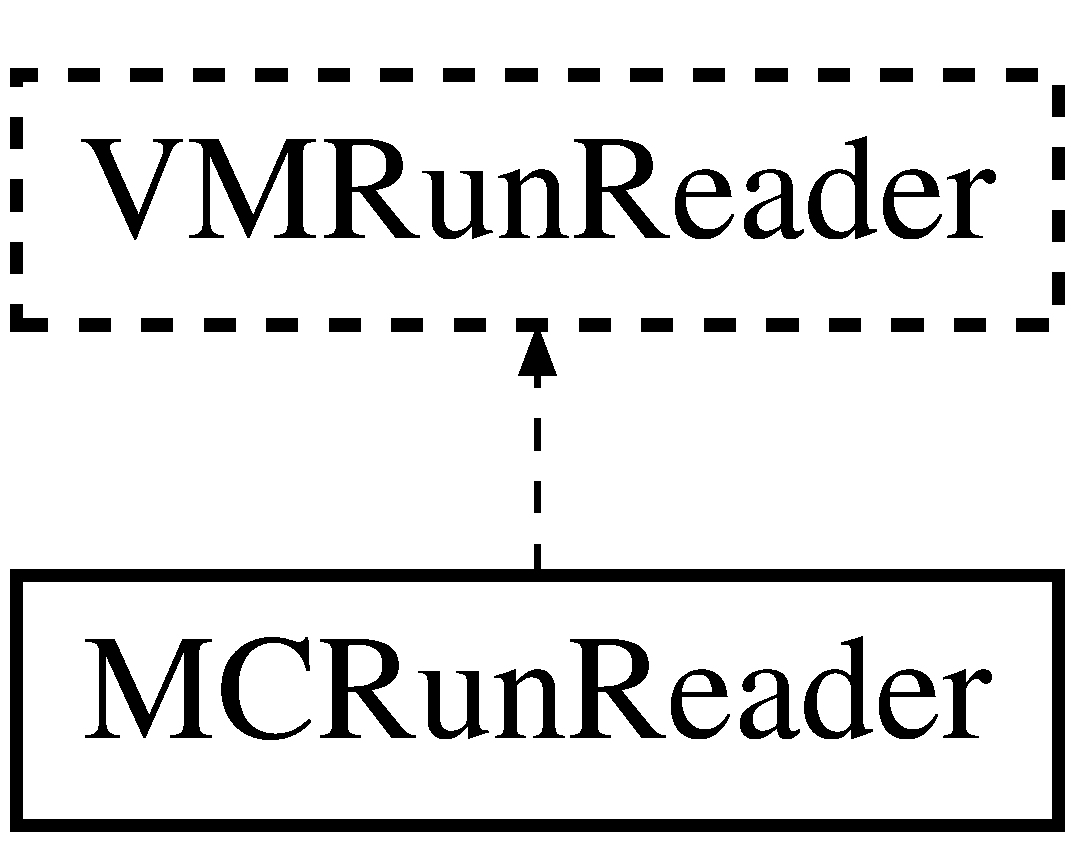
\includegraphics[height=2.000000cm]{class_m_c_run_reader}
\end{center}
\end{figure}
\subsection*{Protected Member Functions}
\begin{DoxyCompactItemize}
\item 
\hyperlink{class_v_m_run_reader_aa84c99e50235a10f563b3487b3930602}{Run\+Data} \hyperlink{class_m_c_run_reader_a1ff16203c127ce8158a9d490ea25ebd3}{Read\+Run\+Data} (const std\+::string \&k\+C\+Run\+Directory) const 
\begin{DoxyCompactList}\small\item\em reads one run from the Nevis dat file located at k\+Dat\+Path. \end{DoxyCompactList}\end{DoxyCompactItemize}
\subsection*{Additional Inherited Members}


\subsection{Detailed Description}
mixin class to read a single run from a R\+O\+O\+T single-\/histogram C macro 

\subsection{Member Function Documentation}
\hypertarget{class_m_c_run_reader_a1ff16203c127ce8158a9d490ea25ebd3}{\index{M\+C\+Run\+Reader@{M\+C\+Run\+Reader}!Read\+Run\+Data@{Read\+Run\+Data}}
\index{Read\+Run\+Data@{Read\+Run\+Data}!M\+C\+Run\+Reader@{M\+C\+Run\+Reader}}
\subsubsection[{Read\+Run\+Data}]{\setlength{\rightskip}{0pt plus 5cm}{\bf M\+C\+Run\+Reader\+::\+Run\+Data} M\+C\+Run\+Reader\+::\+Read\+Run\+Data (
\begin{DoxyParamCaption}
\item[{const std\+::string \&}]{k\+C\+Run\+Directory}
\end{DoxyParamCaption}
) const\hspace{0.3cm}{\ttfamily [protected]}, {\ttfamily [virtual]}}}\label{class_m_c_run_reader_a1ff16203c127ce8158a9d490ea25ebd3}


reads one run from the Nevis dat file located at k\+Dat\+Path. 



Implements \hyperlink{class_v_m_run_reader_afe0f812890dcb11638a66c878f0d8765}{V\+M\+Run\+Reader}.



The documentation for this class was generated from the following files\+:\begin{DoxyCompactItemize}
\item 
src/captain\+Diagnostic/plot\+Planes/\hyperlink{_m_c_run_reader_8h}{M\+C\+Run\+Reader.\+h}\item 
src/captain\+Diagnostic/plot\+Planes/\hyperlink{_m_c_run_reader_8cpp}{M\+C\+Run\+Reader.\+cpp}\end{DoxyCompactItemize}

\hypertarget{class_m_dat_run_reader}{\section{M\+Dat\+Run\+Reader Class Reference}
\label{class_m_dat_run_reader}\index{M\+Dat\+Run\+Reader@{M\+Dat\+Run\+Reader}}
}


mixin class to read a single run in the Nevis dat format  




{\ttfamily \#include $<$M\+Dat\+Run\+Reader.\+h$>$}

Inheritance diagram for M\+Dat\+Run\+Reader\+:\begin{figure}[H]
\begin{center}
\leavevmode
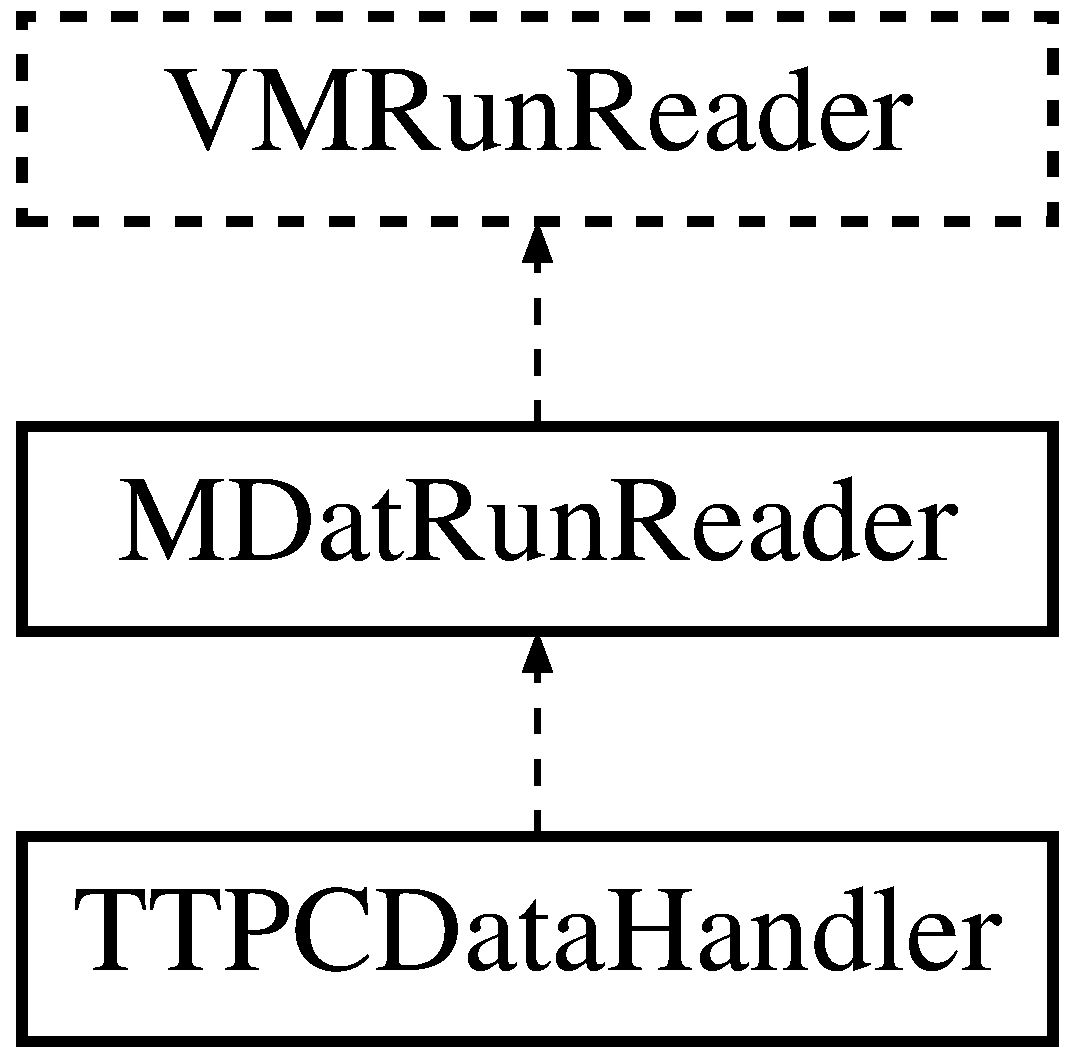
\includegraphics[height=3.000000cm]{class_m_dat_run_reader}
\end{center}
\end{figure}
\subsection*{Protected Member Functions}
\begin{DoxyCompactItemize}
\item 
\hyperlink{class_v_m_run_reader_aa84c99e50235a10f563b3487b3930602}{Run\+Data} \hyperlink{class_m_dat_run_reader_ad9693d690fe452e2839bffe917d0ae41}{Read\+Run\+Data} (const std\+::string \&k\+Dat\+Path) const 
\begin{DoxyCompactList}\small\item\em reads one run from the Nevis dat file located at k\+Dat\+Path. \end{DoxyCompactList}\end{DoxyCompactItemize}
\subsection*{Additional Inherited Members}


\subsection{Detailed Description}
mixin class to read a single run in the Nevis dat format 

\subsection{Member Function Documentation}
\hypertarget{class_m_dat_run_reader_ad9693d690fe452e2839bffe917d0ae41}{\index{M\+Dat\+Run\+Reader@{M\+Dat\+Run\+Reader}!Read\+Run\+Data@{Read\+Run\+Data}}
\index{Read\+Run\+Data@{Read\+Run\+Data}!M\+Dat\+Run\+Reader@{M\+Dat\+Run\+Reader}}
\subsubsection[{Read\+Run\+Data}]{\setlength{\rightskip}{0pt plus 5cm}{\bf Run\+Data} M\+Dat\+Run\+Reader\+::\+Read\+Run\+Data (
\begin{DoxyParamCaption}
\item[{const std\+::string \&}]{k\+Dat\+Path}
\end{DoxyParamCaption}
) const\hspace{0.3cm}{\ttfamily [protected]}, {\ttfamily [virtual]}}}\label{class_m_dat_run_reader_ad9693d690fe452e2839bffe917d0ae41}


reads one run from the Nevis dat file located at k\+Dat\+Path. 



Implements \hyperlink{class_v_m_run_reader_afe0f812890dcb11638a66c878f0d8765}{V\+M\+Run\+Reader}.



The documentation for this class was generated from the following file\+:\begin{DoxyCompactItemize}
\item 
src/daine/captain\+Diagnostic/plot\+Planes/\hyperlink{_m_dat_run_reader_8h}{M\+Dat\+Run\+Reader.\+h}\end{DoxyCompactItemize}

\hypertarget{class_t_t_p_c_data_handler}{\section{T\+T\+P\+C\+Data\+Handler Class Reference}
\label{class_t_t_p_c_data_handler}\index{T\+T\+P\+C\+Data\+Handler@{T\+T\+P\+C\+Data\+Handler}}
}


class to assemble T\+P\+C run data, calculate noise R\+M\+S, and map onto the wire planes  




{\ttfamily \#include $<$T\+T\+P\+C\+Data\+Handler.\+h$>$}

Inheritance diagram for T\+T\+P\+C\+Data\+Handler\+:\begin{figure}[H]
\begin{center}
\leavevmode
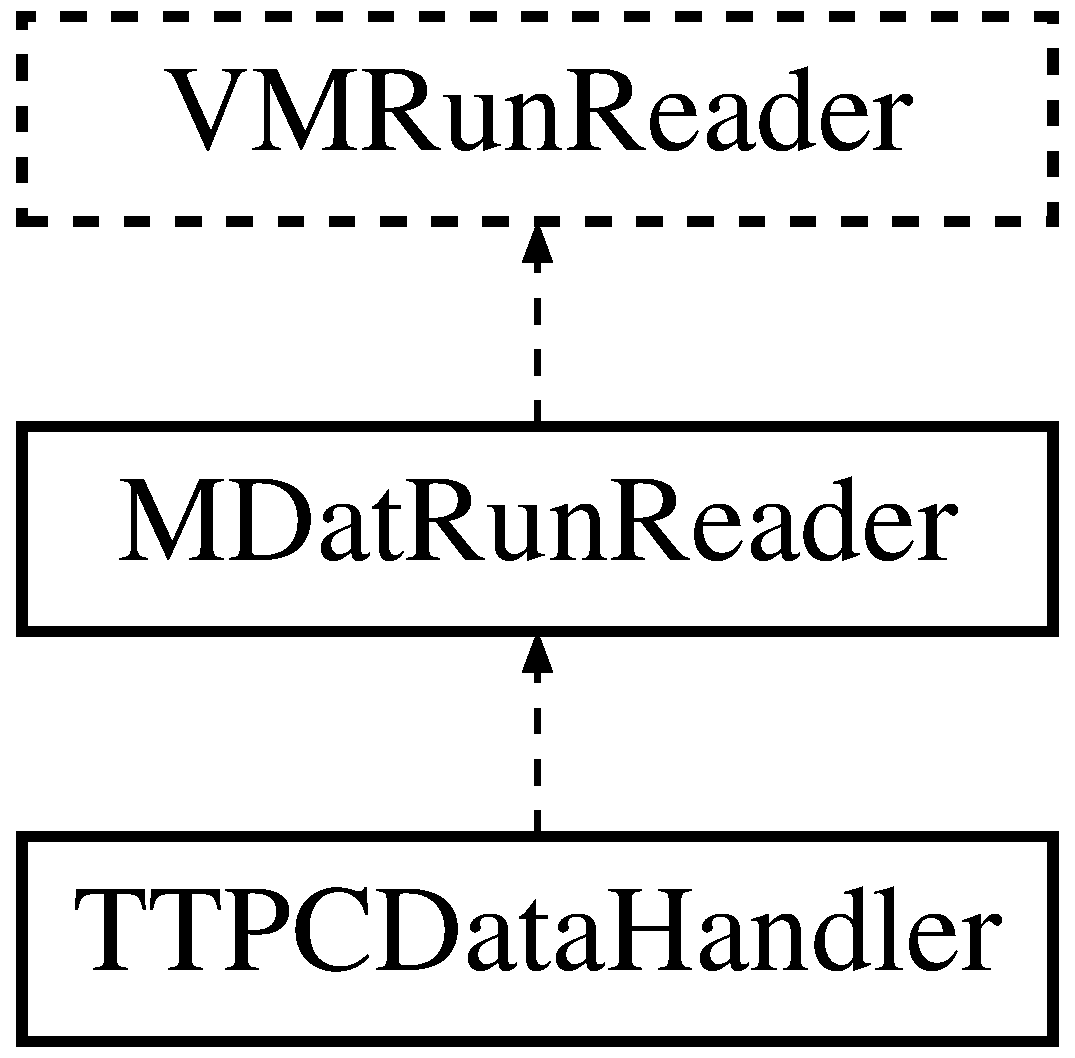
\includegraphics[height=3.000000cm]{class_t_t_p_c_data_handler}
\end{center}
\end{figure}
\subsection*{Public Member Functions}
\begin{DoxyCompactItemize}
\item 
\hyperlink{class_t_t_p_c_data_handler_a65054f0c9a7335a2305de5b63bb84e29}{T\+T\+P\+C\+Data\+Handler} (const std\+::string \&k\+Log\+Path, const std\+::string \&k\+Runs\+Directory, const unsigned k\+First\+Run, const unsigned k\+Last\+Run)
\item 
float \hyperlink{class_t_t_p_c_data_handler_a20538b2bfdb076b6e75bf768d3443f3f}{Compute\+Wire\+Mean\+Voltage} (const unsigned short ki\+Plane, const unsigned short ki\+Wire) const 
\begin{DoxyCompactList}\small\item\em compute the mean sample value on the wire i\+Wire \end{DoxyCompactList}\item 
float \hyperlink{class_t_t_p_c_data_handler_a184f9c2fc4e0cd82cb175624e3e89aaf}{Compute\+Plane\+Collection\+Mean\+Voltage} (const unsigned short ki\+Plane, const unsigned short ki\+Collection) const 
\begin{DoxyCompactList}\small\item\em compute the mean sample value of the entire plane ki\+Plane for collection ki\+Collection \end{DoxyCompactList}\item 
Wires\+R\+M\+S \hyperlink{class_t_t_p_c_data_handler_a0d312c907232f89d96f96ef4dce4a25c}{Get\+Wires\+R\+M\+S} () const 
\item 
A\+S\+I\+Cs\+Mean\+R\+M\+S \hyperlink{class_t_t_p_c_data_handler_a19588e4052efb2c1906384ebf8bad219}{Get\+A\+S\+I\+Cs\+Mean\+R\+M\+S} () const 
\begin{DoxyCompactList}\small\item\em Get the mean R\+M\+S for each A\+S\+I\+C. \end{DoxyCompactList}\item 
Planes\+Data \hyperlink{class_t_t_p_c_data_handler_aa6366249487ef9fc7cd704da7a0fb11f}{Get\+Planes\+Data} () const 
\begin{DoxyCompactList}\small\item\em get all wire plane voltage data \end{DoxyCompactList}\item 
std\+::string \hyperlink{class_t_t_p_c_data_handler_a5e2bb6358b967f29aa1e5e72e286df4a}{Write\+Planes\+Data} (const std\+::string \&k\+R\+O\+O\+T\+Filename) const 
\item 
T\+Canvas \hyperlink{class_t_t_p_c_data_handler_a9d6593f7367185252aaac9ad0290c8f7}{Get\+Voltage\+Histogram} () const 
\begin{DoxyCompactList}\small\item\em constructs a voltage map for each wire plane \end{DoxyCompactList}\item 
T\+H1\+D \hyperlink{class_t_t_p_c_data_handler_acba4e4d412a5c6b86684ecef640c663c}{Get\+Wires\+R\+M\+S\+Histogram} () const 
\begin{DoxyCompactList}\small\item\em constructs a histogram plotting noise R\+M\+S voltage by wire \end{DoxyCompactList}\item 
T\+H1\+D \hyperlink{class_t_t_p_c_data_handler_a73a4c890154ff9da105a8606630c7500}{Get\+A\+S\+I\+Cs\+Mean\+R\+M\+S\+Histogram} () const 
\begin{DoxyCompactList}\small\item\em constructs a histogram plotting mean noise R\+M\+S voltage by A\+S\+I\+C \end{DoxyCompactList}\end{DoxyCompactItemize}
\subsection*{Additional Inherited Members}


\subsection{Detailed Description}
class to assemble T\+P\+C run data, calculate noise R\+M\+S, and map onto the wire planes 

\subsection{Constructor \& Destructor Documentation}
\hypertarget{class_t_t_p_c_data_handler_a65054f0c9a7335a2305de5b63bb84e29}{\index{T\+T\+P\+C\+Data\+Handler@{T\+T\+P\+C\+Data\+Handler}!T\+T\+P\+C\+Data\+Handler@{T\+T\+P\+C\+Data\+Handler}}
\index{T\+T\+P\+C\+Data\+Handler@{T\+T\+P\+C\+Data\+Handler}!T\+T\+P\+C\+Data\+Handler@{T\+T\+P\+C\+Data\+Handler}}
\subsubsection[{T\+T\+P\+C\+Data\+Handler}]{\setlength{\rightskip}{0pt plus 5cm}T\+T\+P\+C\+Data\+Handler\+::\+T\+T\+P\+C\+Data\+Handler (
\begin{DoxyParamCaption}
\item[{const std\+::string \&}]{k\+Log\+Path, }
\item[{const std\+::string \&}]{k\+Runs\+Directory, }
\item[{const unsigned}]{k\+First\+Run, }
\item[{const unsigned}]{k\+Last\+Run}
\end{DoxyParamCaption}
)}}\label{class_t_t_p_c_data_handler_a65054f0c9a7335a2305de5b63bb84e29}
given the path to a log file k\+Log\+Path and the run numbers of the first and last run to be included from this run, k\+First\+Run and k\+Last\+Run, construct a \hyperlink{class_t_t_p_c_data_handler}{T\+T\+P\+C\+Data\+Handler}.

log files should be plaintext formatted as follows\+:

run\+Number; line\+Driver\+Port\+Number1, line\+Driver\+Port\+Number2, ... \# comment \subsection*{comment}

\subsection{Member Function Documentation}
\hypertarget{class_t_t_p_c_data_handler_a184f9c2fc4e0cd82cb175624e3e89aaf}{\index{T\+T\+P\+C\+Data\+Handler@{T\+T\+P\+C\+Data\+Handler}!Compute\+Plane\+Collection\+Mean\+Voltage@{Compute\+Plane\+Collection\+Mean\+Voltage}}
\index{Compute\+Plane\+Collection\+Mean\+Voltage@{Compute\+Plane\+Collection\+Mean\+Voltage}!T\+T\+P\+C\+Data\+Handler@{T\+T\+P\+C\+Data\+Handler}}
\subsubsection[{Compute\+Plane\+Collection\+Mean\+Voltage}]{\setlength{\rightskip}{0pt plus 5cm}float T\+T\+P\+C\+Data\+Handler\+::\+Compute\+Plane\+Collection\+Mean\+Voltage (
\begin{DoxyParamCaption}
\item[{const unsigned short}]{ki\+Plane, }
\item[{const unsigned short}]{ki\+Collection}
\end{DoxyParamCaption}
) const}}\label{class_t_t_p_c_data_handler_a184f9c2fc4e0cd82cb175624e3e89aaf}


compute the mean sample value of the entire plane ki\+Plane for collection ki\+Collection 

\hypertarget{class_t_t_p_c_data_handler_a20538b2bfdb076b6e75bf768d3443f3f}{\index{T\+T\+P\+C\+Data\+Handler@{T\+T\+P\+C\+Data\+Handler}!Compute\+Wire\+Mean\+Voltage@{Compute\+Wire\+Mean\+Voltage}}
\index{Compute\+Wire\+Mean\+Voltage@{Compute\+Wire\+Mean\+Voltage}!T\+T\+P\+C\+Data\+Handler@{T\+T\+P\+C\+Data\+Handler}}
\subsubsection[{Compute\+Wire\+Mean\+Voltage}]{\setlength{\rightskip}{0pt plus 5cm}float T\+T\+P\+C\+Data\+Handler\+::\+Compute\+Wire\+Mean\+Voltage (
\begin{DoxyParamCaption}
\item[{const unsigned short}]{ki\+Plane, }
\item[{const unsigned short}]{ki\+Wire}
\end{DoxyParamCaption}
) const}}\label{class_t_t_p_c_data_handler_a20538b2bfdb076b6e75bf768d3443f3f}


compute the mean sample value on the wire i\+Wire 

\hypertarget{class_t_t_p_c_data_handler_a19588e4052efb2c1906384ebf8bad219}{\index{T\+T\+P\+C\+Data\+Handler@{T\+T\+P\+C\+Data\+Handler}!Get\+A\+S\+I\+Cs\+Mean\+R\+M\+S@{Get\+A\+S\+I\+Cs\+Mean\+R\+M\+S}}
\index{Get\+A\+S\+I\+Cs\+Mean\+R\+M\+S@{Get\+A\+S\+I\+Cs\+Mean\+R\+M\+S}!T\+T\+P\+C\+Data\+Handler@{T\+T\+P\+C\+Data\+Handler}}
\subsubsection[{Get\+A\+S\+I\+Cs\+Mean\+R\+M\+S}]{\setlength{\rightskip}{0pt plus 5cm}T\+T\+P\+C\+Data\+Handler\+::\+A\+S\+I\+Cs\+Mean\+R\+M\+S T\+T\+P\+C\+Data\+Handler\+::\+Get\+A\+S\+I\+Cs\+Mean\+R\+M\+S (
\begin{DoxyParamCaption}
{}
\end{DoxyParamCaption}
) const}}\label{class_t_t_p_c_data_handler_a19588e4052efb2c1906384ebf8bad219}


Get the mean R\+M\+S for each A\+S\+I\+C. 

\hypertarget{class_t_t_p_c_data_handler_a73a4c890154ff9da105a8606630c7500}{\index{T\+T\+P\+C\+Data\+Handler@{T\+T\+P\+C\+Data\+Handler}!Get\+A\+S\+I\+Cs\+Mean\+R\+M\+S\+Histogram@{Get\+A\+S\+I\+Cs\+Mean\+R\+M\+S\+Histogram}}
\index{Get\+A\+S\+I\+Cs\+Mean\+R\+M\+S\+Histogram@{Get\+A\+S\+I\+Cs\+Mean\+R\+M\+S\+Histogram}!T\+T\+P\+C\+Data\+Handler@{T\+T\+P\+C\+Data\+Handler}}
\subsubsection[{Get\+A\+S\+I\+Cs\+Mean\+R\+M\+S\+Histogram}]{\setlength{\rightskip}{0pt plus 5cm}T\+H1\+D T\+T\+P\+C\+Data\+Handler\+::\+Get\+A\+S\+I\+Cs\+Mean\+R\+M\+S\+Histogram (
\begin{DoxyParamCaption}
{}
\end{DoxyParamCaption}
) const}}\label{class_t_t_p_c_data_handler_a73a4c890154ff9da105a8606630c7500}


constructs a histogram plotting mean noise R\+M\+S voltage by A\+S\+I\+C 

\hypertarget{class_t_t_p_c_data_handler_aa6366249487ef9fc7cd704da7a0fb11f}{\index{T\+T\+P\+C\+Data\+Handler@{T\+T\+P\+C\+Data\+Handler}!Get\+Planes\+Data@{Get\+Planes\+Data}}
\index{Get\+Planes\+Data@{Get\+Planes\+Data}!T\+T\+P\+C\+Data\+Handler@{T\+T\+P\+C\+Data\+Handler}}
\subsubsection[{Get\+Planes\+Data}]{\setlength{\rightskip}{0pt plus 5cm}Planes\+Data T\+T\+P\+C\+Data\+Handler\+::\+Get\+Planes\+Data (
\begin{DoxyParamCaption}
{}
\end{DoxyParamCaption}
) const}}\label{class_t_t_p_c_data_handler_aa6366249487ef9fc7cd704da7a0fb11f}


get all wire plane voltage data 

\hypertarget{class_t_t_p_c_data_handler_a9d6593f7367185252aaac9ad0290c8f7}{\index{T\+T\+P\+C\+Data\+Handler@{T\+T\+P\+C\+Data\+Handler}!Get\+Voltage\+Histogram@{Get\+Voltage\+Histogram}}
\index{Get\+Voltage\+Histogram@{Get\+Voltage\+Histogram}!T\+T\+P\+C\+Data\+Handler@{T\+T\+P\+C\+Data\+Handler}}
\subsubsection[{Get\+Voltage\+Histogram}]{\setlength{\rightskip}{0pt plus 5cm}T\+Canvas T\+T\+P\+C\+Data\+Handler\+::\+Get\+Voltage\+Histogram (
\begin{DoxyParamCaption}
{}
\end{DoxyParamCaption}
) const}}\label{class_t_t_p_c_data_handler_a9d6593f7367185252aaac9ad0290c8f7}


constructs a voltage map for each wire plane 

\hypertarget{class_t_t_p_c_data_handler_a0d312c907232f89d96f96ef4dce4a25c}{\index{T\+T\+P\+C\+Data\+Handler@{T\+T\+P\+C\+Data\+Handler}!Get\+Wires\+R\+M\+S@{Get\+Wires\+R\+M\+S}}
\index{Get\+Wires\+R\+M\+S@{Get\+Wires\+R\+M\+S}!T\+T\+P\+C\+Data\+Handler@{T\+T\+P\+C\+Data\+Handler}}
\subsubsection[{Get\+Wires\+R\+M\+S}]{\setlength{\rightskip}{0pt plus 5cm}T\+T\+P\+C\+Data\+Handler\+::\+Wires\+R\+M\+S T\+T\+P\+C\+Data\+Handler\+::\+Get\+Wires\+R\+M\+S (
\begin{DoxyParamCaption}
{}
\end{DoxyParamCaption}
) const}}\label{class_t_t_p_c_data_handler_a0d312c907232f89d96f96ef4dce4a25c}
Calculate the voltage noise R\+M\+S for all wires. This makes two passes\+: one pass calculates an initial voltage pedestal (mean0) and noise R\+M\+S (R\+M\+S0). The second pass recalculates a new pedestal (mean1) and R\+M\+S (R\+M\+S1) excluding bins deviating by more than 3$\ast$\+R\+M\+S0 from mean0. R\+M\+S1 is the final result. \hypertarget{class_t_t_p_c_data_handler_acba4e4d412a5c6b86684ecef640c663c}{\index{T\+T\+P\+C\+Data\+Handler@{T\+T\+P\+C\+Data\+Handler}!Get\+Wires\+R\+M\+S\+Histogram@{Get\+Wires\+R\+M\+S\+Histogram}}
\index{Get\+Wires\+R\+M\+S\+Histogram@{Get\+Wires\+R\+M\+S\+Histogram}!T\+T\+P\+C\+Data\+Handler@{T\+T\+P\+C\+Data\+Handler}}
\subsubsection[{Get\+Wires\+R\+M\+S\+Histogram}]{\setlength{\rightskip}{0pt plus 5cm}T\+H1\+D T\+T\+P\+C\+Data\+Handler\+::\+Get\+Wires\+R\+M\+S\+Histogram (
\begin{DoxyParamCaption}
{}
\end{DoxyParamCaption}
) const}}\label{class_t_t_p_c_data_handler_acba4e4d412a5c6b86684ecef640c663c}


constructs a histogram plotting noise R\+M\+S voltage by wire 

\hypertarget{class_t_t_p_c_data_handler_a5e2bb6358b967f29aa1e5e72e286df4a}{\index{T\+T\+P\+C\+Data\+Handler@{T\+T\+P\+C\+Data\+Handler}!Write\+Planes\+Data@{Write\+Planes\+Data}}
\index{Write\+Planes\+Data@{Write\+Planes\+Data}!T\+T\+P\+C\+Data\+Handler@{T\+T\+P\+C\+Data\+Handler}}
\subsubsection[{Write\+Planes\+Data}]{\setlength{\rightskip}{0pt plus 5cm}std\+::string T\+T\+P\+C\+Data\+Handler\+::\+Write\+Planes\+Data (
\begin{DoxyParamCaption}
\item[{const std\+::string \&}]{k\+R\+O\+O\+T\+Filename}
\end{DoxyParamCaption}
) const}}\label{class_t_t_p_c_data_handler_a5e2bb6358b967f29aa1e5e72e286df4a}
write out all data for all wire planes to a R\+O\+O\+T file, grouped by collection number, an arbitrary association when planes are split across multiple runs. 

The documentation for this class was generated from the following files\+:\begin{DoxyCompactItemize}
\item 
src/captain\+Diagnostic/plot\+Planes/\hyperlink{_t_t_p_c_data_handler_8h}{T\+T\+P\+C\+Data\+Handler.\+h}\item 
src/captain\+Diagnostic/plot\+Planes/\hyperlink{_t_t_p_c_data_handler_8cpp}{T\+T\+P\+C\+Data\+Handler.\+cpp}\end{DoxyCompactItemize}

\hypertarget{class_v_m_run_reader}{\section{V\+M\+Run\+Reader Class Reference}
\label{class_v_m_run_reader}\index{V\+M\+Run\+Reader@{V\+M\+Run\+Reader}}
}


abstract base class for mixins that read various run data files.  




{\ttfamily \#include $<$V\+M\+Run\+Reader.\+h$>$}

Inheritance diagram for V\+M\+Run\+Reader\+:\begin{figure}[H]
\begin{center}
\leavevmode
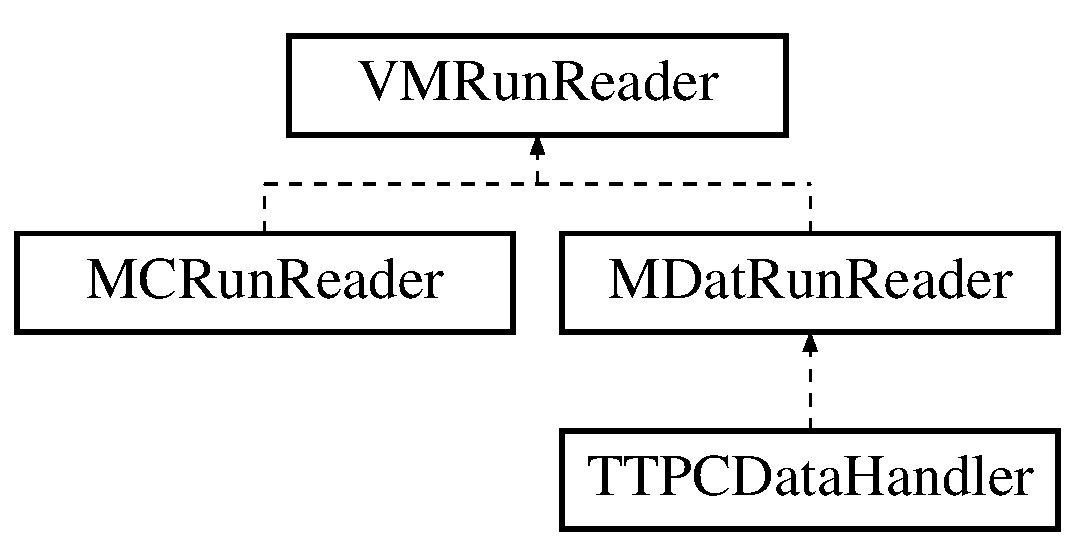
\includegraphics[height=3.000000cm]{class_v_m_run_reader}
\end{center}
\end{figure}
\subsection*{Public Member Functions}
\begin{DoxyCompactItemize}
\item 
virtual \hyperlink{class_v_m_run_reader_aa84c99e50235a10f563b3487b3930602}{Run\+Data} \hyperlink{class_v_m_run_reader_afe0f812890dcb11638a66c878f0d8765}{Read\+Run\+Data} (const std\+::string \&k\+Path) const =0
\begin{DoxyCompactList}\small\item\em Reads one run. \end{DoxyCompactList}\end{DoxyCompactItemize}
\subsection*{Protected Types}
\begin{DoxyCompactItemize}
\item 
typedef std\+::array$<$ std\+::array\\*
$<$ int, kg\+N\+Samples\+Per\+Channel $>$\\*
, kg\+N\+Channels\+Per\+Run $>$ \hyperlink{class_v_m_run_reader_aca02fe95a36b6651ad0cf4bc7a8d02e4}{Run\+Collection}
\item 
typedef std\+::vector\\*
$<$ \hyperlink{class_v_m_run_reader_aca02fe95a36b6651ad0cf4bc7a8d02e4}{Run\+Collection} $>$ \hyperlink{class_v_m_run_reader_aa84c99e50235a10f563b3487b3930602}{Run\+Data}
\end{DoxyCompactItemize}
\subsection*{Static Protected Member Functions}
\begin{DoxyCompactItemize}
\item 
static std\+::string \hyperlink{class_v_m_run_reader_aa073a42cf6eadf42fd9937d8c8f24dae}{P\+O\+S\+I\+X\+Expand} (const std\+::string \&k\+Word)
\begin{DoxyCompactList}\small\item\em expands a P\+O\+S\+I\+X expression, i.\+e., a path containing environmental variables \end{DoxyCompactList}\end{DoxyCompactItemize}


\subsection{Detailed Description}
abstract base class for mixins that read various run data files. 

\subsection{Member Typedef Documentation}
\hypertarget{class_v_m_run_reader_aca02fe95a36b6651ad0cf4bc7a8d02e4}{\index{V\+M\+Run\+Reader@{V\+M\+Run\+Reader}!Run\+Collection@{Run\+Collection}}
\index{Run\+Collection@{Run\+Collection}!V\+M\+Run\+Reader@{V\+M\+Run\+Reader}}
\subsubsection[{Run\+Collection}]{\setlength{\rightskip}{0pt plus 5cm}typedef std\+::array$<$std\+::array$<$int, kg\+N\+Samples\+Per\+Channel$>$, kg\+N\+Channels\+Per\+Run$>$ {\bf V\+M\+Run\+Reader\+::\+Run\+Collection}\hspace{0.3cm}{\ttfamily [protected]}}}\label{class_v_m_run_reader_aca02fe95a36b6651ad0cf4bc7a8d02e4}
Run\+Data\+: \mbox{[}collection\mbox{]}\mbox{[}channel\mbox{]}\mbox{[}sample\mbox{]} stores one run's data, indexed by collection, channel, and sample. \hypertarget{class_v_m_run_reader_aa84c99e50235a10f563b3487b3930602}{\index{V\+M\+Run\+Reader@{V\+M\+Run\+Reader}!Run\+Data@{Run\+Data}}
\index{Run\+Data@{Run\+Data}!V\+M\+Run\+Reader@{V\+M\+Run\+Reader}}
\subsubsection[{Run\+Data}]{\setlength{\rightskip}{0pt plus 5cm}typedef std\+::vector$<${\bf Run\+Collection}$>$ {\bf V\+M\+Run\+Reader\+::\+Run\+Data}\hspace{0.3cm}{\ttfamily [protected]}}}\label{class_v_m_run_reader_aa84c99e50235a10f563b3487b3930602}


\subsection{Member Function Documentation}
\hypertarget{class_v_m_run_reader_aa073a42cf6eadf42fd9937d8c8f24dae}{\index{V\+M\+Run\+Reader@{V\+M\+Run\+Reader}!P\+O\+S\+I\+X\+Expand@{P\+O\+S\+I\+X\+Expand}}
\index{P\+O\+S\+I\+X\+Expand@{P\+O\+S\+I\+X\+Expand}!V\+M\+Run\+Reader@{V\+M\+Run\+Reader}}
\subsubsection[{P\+O\+S\+I\+X\+Expand}]{\setlength{\rightskip}{0pt plus 5cm}std\+::string V\+M\+Run\+Reader\+::\+P\+O\+S\+I\+X\+Expand (
\begin{DoxyParamCaption}
\item[{const std\+::string \&}]{k\+Word}
\end{DoxyParamCaption}
)\hspace{0.3cm}{\ttfamily [static]}, {\ttfamily [protected]}}}\label{class_v_m_run_reader_aa073a42cf6eadf42fd9937d8c8f24dae}


expands a P\+O\+S\+I\+X expression, i.\+e., a path containing environmental variables 

\hypertarget{class_v_m_run_reader_afe0f812890dcb11638a66c878f0d8765}{\index{V\+M\+Run\+Reader@{V\+M\+Run\+Reader}!Read\+Run\+Data@{Read\+Run\+Data}}
\index{Read\+Run\+Data@{Read\+Run\+Data}!V\+M\+Run\+Reader@{V\+M\+Run\+Reader}}
\subsubsection[{Read\+Run\+Data}]{\setlength{\rightskip}{0pt plus 5cm}virtual {\bf Run\+Data} V\+M\+Run\+Reader\+::\+Read\+Run\+Data (
\begin{DoxyParamCaption}
\item[{const std\+::string \&}]{k\+Path}
\end{DoxyParamCaption}
) const\hspace{0.3cm}{\ttfamily [pure virtual]}}}\label{class_v_m_run_reader_afe0f812890dcb11638a66c878f0d8765}


Reads one run. 



Implemented in \hyperlink{class_m_c_run_reader_a1ff16203c127ce8158a9d490ea25ebd3}{M\+C\+Run\+Reader}, and \hyperlink{class_m_dat_run_reader_ad9693d690fe452e2839bffe917d0ae41}{M\+Dat\+Run\+Reader}.



The documentation for this class was generated from the following files\+:\begin{DoxyCompactItemize}
\item 
src/captain\+Diagnostic/plot\+Planes/\hyperlink{_v_m_run_reader_8h}{V\+M\+Run\+Reader.\+h}\item 
src/captain\+Diagnostic/plot\+Planes/\hyperlink{_v_m_run_reader_8cpp}{V\+M\+Run\+Reader.\+cpp}\end{DoxyCompactItemize}

\chapter{File Documentation}
\hypertarget{_configuration_8h}{\section{src/captain\+Diagnostic/plot\+Planes/\+Configuration.h File Reference}
\label{_configuration_8h}\index{src/captain\+Diagnostic/plot\+Planes/\+Configuration.\+h@{src/captain\+Diagnostic/plot\+Planes/\+Configuration.\+h}}
}
{\ttfamily \#include $<$array$>$}\\*
{\ttfamily \#include $<$string$>$}\\*
\subsection*{Macros}
\begin{DoxyCompactItemize}
\item 
\#define \hyperlink{_configuration_8h_a70325c7e8d5e0c4faf6a55aa93034e71}{C\+\_\+\+M\+A\+C\+R\+O\+\_\+\+M\+O\+D\+E}~0
\end{DoxyCompactItemize}


\subsection{Macro Definition Documentation}
\hypertarget{_configuration_8h_a70325c7e8d5e0c4faf6a55aa93034e71}{\index{Configuration.\+h@{Configuration.\+h}!C\+\_\+\+M\+A\+C\+R\+O\+\_\+\+M\+O\+D\+E@{C\+\_\+\+M\+A\+C\+R\+O\+\_\+\+M\+O\+D\+E}}
\index{C\+\_\+\+M\+A\+C\+R\+O\+\_\+\+M\+O\+D\+E@{C\+\_\+\+M\+A\+C\+R\+O\+\_\+\+M\+O\+D\+E}!Configuration.\+h@{Configuration.\+h}}
\subsubsection[{C\+\_\+\+M\+A\+C\+R\+O\+\_\+\+M\+O\+D\+E}]{\setlength{\rightskip}{0pt plus 5cm}\#define C\+\_\+\+M\+A\+C\+R\+O\+\_\+\+M\+O\+D\+E~0}}\label{_configuration_8h_a70325c7e8d5e0c4faf6a55aa93034e71}
set C\+\_\+\+M\+A\+C\+R\+O\+\_\+\+M\+O\+D\+E to 1 if you want to read from Read\+Data\+By\+Channel R\+O\+O\+T $\ast$.C macro run directories instead of dat files. 
\hypertarget{main_8cpp}{\section{src/daine/captain\+Diagnostic/plot\+Planes/main.cpp File Reference}
\label{main_8cpp}\index{src/daine/captain\+Diagnostic/plot\+Planes/main.\+cpp@{src/daine/captain\+Diagnostic/plot\+Planes/main.\+cpp}}
}
{\ttfamily \#include \char`\"{}T\+T\+P\+C\+Data\+Handler.\+h\char`\"{}}\\*
\subsection*{Functions}
\begin{DoxyCompactItemize}
\item 
int \hyperlink{main_8cpp_ac0f2228420376f4db7e1274f2b41667c}{main} (int argc, const char $\ast$argv\mbox{[}$\,$\mbox{]})
\end{DoxyCompactItemize}


\subsection{Function Documentation}
\hypertarget{main_8cpp_ac0f2228420376f4db7e1274f2b41667c}{\index{main.\+cpp@{main.\+cpp}!main@{main}}
\index{main@{main}!main.\+cpp@{main.\+cpp}}
\subsubsection[{main}]{\setlength{\rightskip}{0pt plus 5cm}int main (
\begin{DoxyParamCaption}
\item[{int}]{argc, }
\item[{const char $\ast$}]{argv\mbox{[}$\,$\mbox{]}}
\end{DoxyParamCaption}
)}}\label{main_8cpp_ac0f2228420376f4db7e1274f2b41667c}

\hypertarget{_m_c_run_reader_8cpp}{\section{src/daine/captain\+Diagnostic/plot\+Planes/\+M\+C\+Run\+Reader.cpp File Reference}
\label{_m_c_run_reader_8cpp}\index{src/daine/captain\+Diagnostic/plot\+Planes/\+M\+C\+Run\+Reader.\+cpp@{src/daine/captain\+Diagnostic/plot\+Planes/\+M\+C\+Run\+Reader.\+cpp}}
}
{\ttfamily \#include \char`\"{}M\+C\+Run\+Reader.\+h\char`\"{}}\\*

\hypertarget{_m_c_run_reader_8h}{\section{src/daine/captain\+Diagnostic/plot\+Planes/\+M\+C\+Run\+Reader.h File Reference}
\label{_m_c_run_reader_8h}\index{src/daine/captain\+Diagnostic/plot\+Planes/\+M\+C\+Run\+Reader.\+h@{src/daine/captain\+Diagnostic/plot\+Planes/\+M\+C\+Run\+Reader.\+h}}
}
{\ttfamily \#include \char`\"{}V\+M\+Run\+Reader.\+h\char`\"{}}\\*
{\ttfamily \#include $<$cstring$>$}\\*
\subsection*{Classes}
\begin{DoxyCompactItemize}
\item 
class \hyperlink{class_m_c_run_reader}{M\+C\+Run\+Reader}
\begin{DoxyCompactList}\small\item\em mixin class to read a single run from a R\+O\+O\+T single-\/histogram C macro \end{DoxyCompactList}\end{DoxyCompactItemize}

\hypertarget{_m_dat_run_reader_8h}{\section{src/daine/captain\+Diagnostic/plot\+Planes/\+M\+Dat\+Run\+Reader.h File Reference}
\label{_m_dat_run_reader_8h}\index{src/daine/captain\+Diagnostic/plot\+Planes/\+M\+Dat\+Run\+Reader.\+h@{src/daine/captain\+Diagnostic/plot\+Planes/\+M\+Dat\+Run\+Reader.\+h}}
}
{\ttfamily \#include \char`\"{}V\+M\+Run\+Reader.\+h\char`\"{}}\\*
\subsection*{Classes}
\begin{DoxyCompactItemize}
\item 
class \hyperlink{class_m_dat_run_reader}{M\+Dat\+Run\+Reader}
\begin{DoxyCompactList}\small\item\em mixin class to read a single run in the Nevis dat format \end{DoxyCompactList}\end{DoxyCompactItemize}

\hypertarget{_t_t_p_c_data_handler_8cpp}{\section{src/captain\+Diagnostic/plot\+Planes/\+T\+T\+P\+C\+Data\+Handler.cpp File Reference}
\label{_t_t_p_c_data_handler_8cpp}\index{src/captain\+Diagnostic/plot\+Planes/\+T\+T\+P\+C\+Data\+Handler.\+cpp@{src/captain\+Diagnostic/plot\+Planes/\+T\+T\+P\+C\+Data\+Handler.\+cpp}}
}
{\ttfamily \#include \char`\"{}T\+T\+P\+C\+Data\+Handler.\+h\char`\"{}}\\*

\hypertarget{_t_t_p_c_data_handler_8h}{\section{src/captain\+Diagnostic/plot\+Planes/\+T\+T\+P\+C\+Data\+Handler.h File Reference}
\label{_t_t_p_c_data_handler_8h}\index{src/captain\+Diagnostic/plot\+Planes/\+T\+T\+P\+C\+Data\+Handler.\+h@{src/captain\+Diagnostic/plot\+Planes/\+T\+T\+P\+C\+Data\+Handler.\+h}}
}
{\ttfamily \#include \char`\"{}M\+Dat\+Run\+Reader.\+h\char`\"{}}\\*
{\ttfamily \#include \char`\"{}M\+C\+Run\+Reader.\+h\char`\"{}}\\*
{\ttfamily \#include $<$T\+H1.\+h$>$}\\*
{\ttfamily \#include $<$T\+H2.\+h$>$}\\*
{\ttfamily \#include $<$T\+File.\+h$>$}\\*
{\ttfamily \#include $<$T\+Directory.\+h$>$}\\*
{\ttfamily \#include $<$T\+Style.\+h$>$}\\*
{\ttfamily \#include $<$T\+Canvas.\+h$>$}\\*
{\ttfamily \#include $<$map$>$}\\*
{\ttfamily \#include $<$set$>$}\\*
{\ttfamily \#include $<$memory$>$}\\*
{\ttfamily \#include $<$cmath$>$}\\*
\subsection*{Classes}
\begin{DoxyCompactItemize}
\item 
class \hyperlink{class_t_t_p_c_data_handler}{T\+T\+P\+C\+Data\+Handler}
\begin{DoxyCompactList}\small\item\em class to assemble T\+P\+C run data, calculate noise R\+M\+S, and map onto the wire planes \end{DoxyCompactList}\end{DoxyCompactItemize}

\hypertarget{_v_m_run_reader_8cpp}{\section{src/captain\+Diagnostic/plot\+Planes/\+V\+M\+Run\+Reader.cpp File Reference}
\label{_v_m_run_reader_8cpp}\index{src/captain\+Diagnostic/plot\+Planes/\+V\+M\+Run\+Reader.\+cpp@{src/captain\+Diagnostic/plot\+Planes/\+V\+M\+Run\+Reader.\+cpp}}
}
{\ttfamily \#include \char`\"{}V\+M\+Run\+Reader.\+h\char`\"{}}\\*

\hypertarget{_v_m_run_reader_8h}{\section{src/captain\+Diagnostic/plot\+Planes/\+V\+M\+Run\+Reader.h File Reference}
\label{_v_m_run_reader_8h}\index{src/captain\+Diagnostic/plot\+Planes/\+V\+M\+Run\+Reader.\+h@{src/captain\+Diagnostic/plot\+Planes/\+V\+M\+Run\+Reader.\+h}}
}
{\ttfamily \#include \char`\"{}Configuration.\+h\char`\"{}}\\*
{\ttfamily \#include $<$array$>$}\\*
{\ttfamily \#include $<$iostream$>$}\\*
{\ttfamily \#include $<$vector$>$}\\*
{\ttfamily \#include $<$string$>$}\\*
{\ttfamily \#include $<$fstream$>$}\\*
{\ttfamily \#include $<$wordexp.\+h$>$}\\*
\subsection*{Classes}
\begin{DoxyCompactItemize}
\item 
class \hyperlink{class_v_m_run_reader}{V\+M\+Run\+Reader}
\end{DoxyCompactItemize}

%--- End generated contents ---

% Index
\newpage
\phantomsection
\addcontentsline{toc}{chapter}{Index}
\printindex

\end{document}
